\documentclass{article}
\usepackage[utf8]{inputenc}
\usepackage[T1]{fontenc}
\usepackage[russian]{babel}
\usepackage{tikz}
\usepackage{graphicx}
\usepackage{titlesec}
\usepackage{amsfonts}
\usepackage{amsmath}
\usepackage[left=2cm,right=2cm,
    top=2cm,bottom=2cm,bindingoffset=0cm]{geometry}
\renewcommand{\thesection}{\arabic{section}}
\titleformat{\section}{\large\bfseries}{\thesection}{1em}{}
\title{Интегрирование}
\author{Каренин Константин Витальевич}
\date{02.04.2024}
\begin{document}

\begin{titlepage}
    \centering
    \vspace*{0.5 cm}
    
    \textsc{\LARGE \textbf{Специальные разделы высшей математики}}
    \vspace{1.5cm}
    
    \rule{\linewidth}{0.2 mm} \\[0.4 cm]
    { \huge \bfseries Линейная алгебра}
    \rule{\linewidth}{0.2 mm} \\[1.5 cm]
    
    \Large Выполнили: \\
    Каренин Константин \\
    Темиров Тимур \\
    Гонин Сергей \\
    Малышева Алиса \\
    
    \vspace{0.5cm}
    
    Группа: М3104
    
    \vspace{0.5cm}
    
    Преподаватель: Сарычев Павел
    
    \vspace{0.5cm}
    
    Университет ИТМО
    
    \vfill

    
\includegraphics[height=70px]{logo.jpg}
    
    2.04.2024
    
\end{titlepage}

\setcounter{page}{2}

% task 1
\newpage
    \section{Евклидовы пространства функций}
    \subsection{}
    \subsubsection{$B = \{1, t, t^2\}$}
    Проверим, что данная система линейно независима:\\
    $P(t)=c_1 + c_2t + c_3t^2 = 0 \; \; \; \forall t \in \mathbb{R}$\\
    $P(0) = 0 \to c_1 = 0$\\
    $P(1) = c_1 + c_2 + c_3 = 0$\\
    $P(-1) = c_1 - c_2 + c_3 = 0$\\
    \begin{equation*}
        \begin{cases}
            c_1 = 0 \\
            c_1 + c_2 + c_3 = 0 \\
            c_1 - c_2 + c_3 = 0 \\
        \end{cases}
        \begin{cases}
            c_1 = 0 \\
            c_3 = -c_2 \\
            -2 c_2 = 0 \\
        \end{cases}
        \begin{cases}
            c_2 = 0 \\
            c_3 = 0 \\
            c_1 = 0 \\
        \end{cases}
        \Rightarrow
    B - \text{линейно независимый} \Rightarrow B - \text{это базис}\\
    \end{equation*}
    Ортогонализируем данный бащис:\\
    Пусть $f_1 = 1, f_2 = f_1 + \alpha t = 1 + \alpha t$\\
    Тогда\\
    $\alpha = - \frac{(f_1, f_1}{(t, f_1)} = - \frac{\int_{-1}^1 dt}{\int_{-1}^1 tdt} = - \frac{2}{0}$ - получился невалидный результат, значит:\\
    $(t, 1) = 0 \Rightarrow t \perp 1$\\ \\
    Пусть $f_3 = f_1 + \alpha t^2 = 1 + \alpha t^2$\\
    $\alpha = - \frac{\int_{-1}^1 dt}{\int_{-1}^1 t^2dt} = - \frac{2}{\frac{2}{3}} = -3$\\
    Тогда $f_3 = 1 - 3t^2$\\
    $(f_3, t) = \int_{-1}^1 (t-3t^2)dt = \frac{1}{2} - \frac{3}{4} - \frac{1}{2} + \frac{3}{4} = 0 \Rightarrow f_3 \perp t$\\
    Тогда $B_H = \{1, t, 1-3t^2\}$
    \subsubsection{$L_n (t) = \frac{1}{2^n n!} \frac{d^n}{dt^n}((t^2-1)n)$}
    $L_0 (t) = 1$\\
    $L_1 (t) = \frac{1}{2} 2t = t$\\
    $L_2 (t) = \frac{1}{8} \frac{d^2}{dt^2}((t^2-1)^2) = \frac{3t^2 - 1}{2} = \frac{3}{2} t^2 - 1$\\
    $L_3 (t) = \frac{1}{48} \frac{d^3}{dt^3}((t^2-1)^3) = \frac{5t^3}{2} - \frac{3}{2}t$\\
    \subsubsection{$L_0 (t) = (1, 0, 0)_{BM}$}
    $L_1 (t) = (0, 1, 0)_{BM}$\\
    $L_2 (t) = (-1, 0, \frac{3}{2})_{BM}$\\
    $L_3 (t) = (0, -\frac{3}{2}, \frac{5}{2}t)_{BM}$\\
    $L_0 \perp L_1$\\
    $(L_1, L_2) = 0 \Rightarrow L_2 \perp L_1$\\
    $(L_0, L_2) = -1 \Rightarrow L_0 \; \text{не ортогонален} \; L_1$\\
    $(L_3, L_2) = \frac{15}{4}t - \text{об ортогональности можно говорить исходя из } t$\\
    Система $\{L_0, L_1, L_2, L_2, L_3\} - $ не ортогональна
    \subsubsection{$P_3(t) =  t^3 - 2t^2 + t + 1$}
    $P_3 (t) = \frac{2}{5}L_3(t)- \frac{4}{3}L_2(t) + 1\frac{3}{5}L_1(t) + 2\frac{1}{3}L_0(t) = (\frac{2}{5}, -\frac{4}{3}, 1\frac{3}{5}, 2\frac{1}{3})_L$
    \subsection{}
    \subsubsection{}
    $\int_{-\pi}^\pi \cos mx \sin kx \; dx = \frac{1}{2} \int_{-\pi}^\pi (\sin(kx - mx) + \sin(kx + mx)) \; dx = \int_{0}^\pi \sin(kx-mx) \; dx + \int_{0}^\pi \sin(kx+mx) \; dx = 0$, \\
    т.к. $\int_{0}^\pi \sin mx \; dx = 2(\frac{\cos m \pi}{m} - \frac{\cos 0}{m}) = 0$\\
    $\int_{-\pi}^\pi \cos mx \cos kx \; dx = \int_{0}^\pi \cos(mx-kx) \; dx + \int_{0}^\pi \cos (mx-kx) = 0$, \\
    т.к. $\int_{-\pi}^\pi \cos mx \; dx = 2(\frac{\sin m \pi}{m} - \frac{\sin 0}{m}) = 0$\\
    $\int_{-\pi}^\pi \sin mx \sin kx \; dx = \int_{0}^\pi \cos(mx-kx) \; dx - \int_{0}^\pi \cos (mx+kx) \; dx = 0$\\
    следовательно всё со всем ортогонально, т.к. скаляры произведения всех векторов множества равны 0.\\
    $|| \cos mx || = \sqrt{\int_{-\pi}^\pi \cos^2 mx \; dx} = \sqrt{2\int_{0}^\pi \cos^2 mx \; dx }= \sqrt{\int_{0}^\pi 2\cos^2 mx \; dx }= \sqrt{\int_{0}^\pi (\cos 2mx + 1)\; dx} = \sqrt{\int_{0}^\pi dx} = \sqrt{\pi}$\\
    $|| \sin mx || = \sqrt{\int_{-\pi}^\pi \sin^2 mx \; dx} = \sqrt{\int_{-\pi}^\pi \frac{1 - \cos 2mx}{2} \; dx} = \sqrt{\pi}$\\
    $||1|| = \sqrt{\int_{-\pi}^\pi \; dx} = \sqrt{2 \pi}$, тогда \\
    $N = \{\frac{1}{\sqrt{2\pi}}, \frac{\sin x}{\sqrt{\pi}}, \frac{\cos x}{\pi}, ... , \frac{\sin mx}{\sqrt{\pi}}, \frac{\cos mx}{\sqrt{\pi}}\} -$ ортонормированная система
    \subsubsection{$f(x) = 2x$}
    $Pr_1 2x = \frac{\int_{-\pi}^\pi 2x \; dx}{\sqrt{\int_{-\pi}^\pi dx}} = 0$\\
    $Pr_{\cos mx} 2x = \frac{\int_{-\pi}^\pi 2x \cos mx \; dx}{\sqrt{\pi}} = 0$\\
    $\sin x$ симетричен на $[-\pi;\pi]$ относительно $0$\\
    $Pr_{\sin mx} 2x = \frac{2 \int_{-\pi}^\pi x \sin mx \; dx}{\sqrt{\pi}} = \frac{2}{\sqrt{\pi}} \frac{-2 \pi m \cos m \pi + 2 \sin m \pi}{m^2}$
    \subsubsection{$f(x) \sim \frac{a_0}{2} + \sum_{n=1}^{\infty}(a_u \cos mx + bm sin mx)$}
    $a_0 = \frac{1}{\pi} \int_{-\pi}^\pi 2x \; dx = 0$\\
    $a_m = \frac{1}{\pi} \int_{-\pi}^\pi 2x \cos mx \; dx = 0$\\
    $b_m = \frac{1}{\pi} \int_{-\pi}^\pi 2x \sin mx \; dx = \frac{-4\pi m \cos(\pi m) + 4 \sin (\pi m)}{\pi m^2}$\\
    $f(x) \sim \frac{a_0}{2} + \sum_{n=1}^{\infty}(\frac{-4\pi m \cos(\pi m) + 4 \sin (\pi m)}{\pi m^2})$
    
    \subsubsection{}
    \begin{equation*}
        n = 5 \; \; \; \; \; \; \; \; \; \; \; \; \; \; \; \; \; \;
        \; \; \; \; \; \; \; \; \;
        n = 10 \; \; \; \; \; \; \; \; \; \; \; \; \; \; \; \; \; \;
        \; \; \; \; \; \; \; \; \;
        n = 15 \; \; \; \; \; \; \; \; \; \; \; \; \; \; \; \; \; \;
        \; \; \; \; \; \; \; \; \;
        n = \infty
    \end{equation*}
    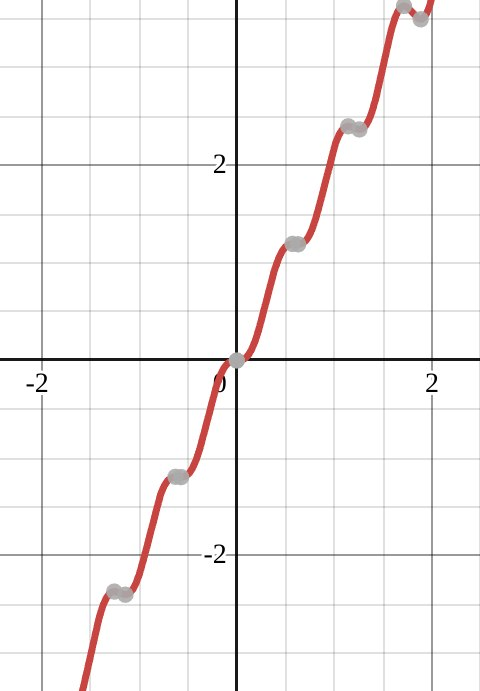
\includegraphics[height=200px]{rgr1.1.jpg}
    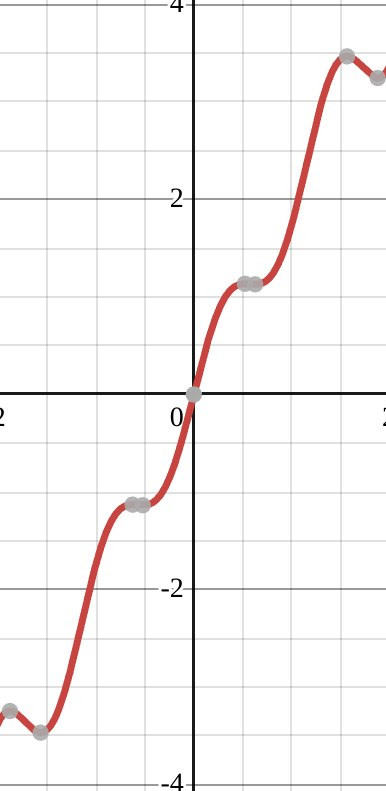
\includegraphics[height=200px]{rgr1.2.jpg}
    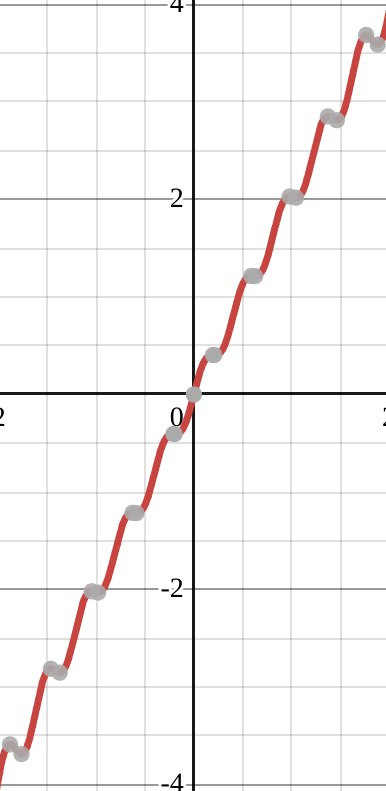
\includegraphics[height=200px]{rgr1.3.jpg}
    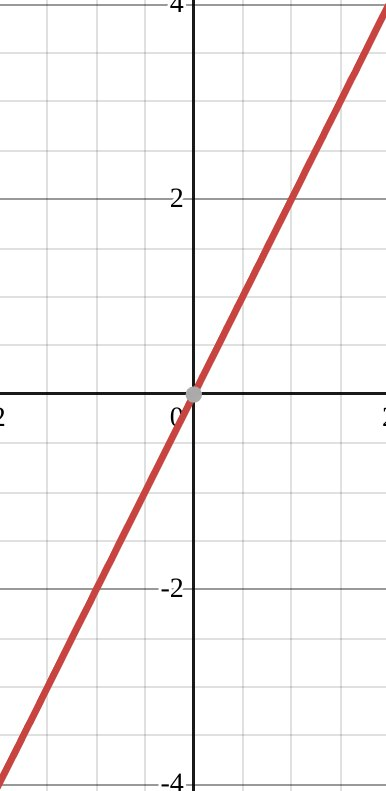
\includegraphics[height=200px]{rgr1.4.jpg}
    \subsubsection{Вывод}
    Чем больше $n$, тем "ближе" \; ряд Фурье сходится к изначальной функции на $[-\pi;\pi]$, тем самым $n$ "сглаживает"
    
    
    
    

    
% task 2
\newpage
    \section{Приведение уравнения поверхности 2-го порядка к каноническому виду}
    $2x^2 - bxy + 2y^2 + z^2 - 25 = 0$
    \subsection{$F(x, y, z) = 2x^2 -bxy + 2\phi^2 + z^2$}
    \begin{equation*}
    A = 
        \begin{pmatrix}
            2& -3& 0\\
            -3& 2& 0\\
            0& 0& 1\\
        \end{pmatrix}
    \end{equation*}
    Собственные числа и векторы:
    \begin{equation*}
        \lambda_1 = -1 \; \; \; \; \; \; 
        \widetilde{v_1}=
        \begin{pmatrix}
            1\\
            1\\
            0\\
        \end{pmatrix}
    \end{equation*}
    \begin{equation*}
        \lambda_2 = 1 \; \; \; \; \; \; 
        \widetilde{v_2}=
        \begin{pmatrix}
            0\\
            0\\
            1\\
        \end{pmatrix}
    \end{equation*}
    \begin{equation*}
        \lambda_3 = 5 \; \; \; \; \; \; 
        \widetilde{v_3}=
        \begin{pmatrix}
            -1\\
            1\\
            0\\
        \end{pmatrix}
    \end{equation*}
    \begin{equation*}
        \begin{cases}
            v_1=
            \begin{pmatrix}
                \frac{1}{\sqrt{2}}\\
                \frac{1}{\sqrt{2}}\\
                0\\
            \end{pmatrix}\\
            v_2=
            \begin{pmatrix}
                0\\
                0\\
                1\\
            \end{pmatrix}\\
            v_3=
            \begin{pmatrix}
                -\frac{1}{\sqrt{2}}\\
                \frac{1}{\sqrt{2}}\\
                0\\
            \end{pmatrix}\\
        \end{cases} - \text{ортонормированный базис}
    \end{equation*}
    $\{e_1, e_2, e_3\} = \{i, j, k\}$\\
    $\forall u \in \mathbb{R} \; \; \; \;$
    $u_e = T_{e \to v} u_v$ \\
    \begin{equation*}
        \begin{pmatrix}
            x\\
            y\\
            z\\
        \end{pmatrix}
        =
        \begin{pmatrix}
            \frac{1}{\sqrt{2}}& 0& - \frac{1}{\sqrt{2}}\\
            \frac{1}{\sqrt{2}}& 0& \frac{1}{\sqrt{2}}\\
            0& 1& 0\\
        \end{pmatrix}
        \begin{pmatrix}
            x'\\
            y'\\
            z'\\
        \end{pmatrix}
    \end{equation*}
    \begin{equation*}
        \begin{cases}
            x = \frac{1}{\sqrt{2}}x' - \frac{1}{\sqrt{2}}z'\\
            y = \frac{1}{\sqrt{2}}x' + \frac{1}{\sqrt{2}}z'\\
            z = y'\\
        \end{cases}
    \end{equation*}
    \begin{equation*}
        \begin{pmatrix}
            -1& 0& 9\\
            0& 1& 0\\
            0& 0& 5\\
        \end{pmatrix}
        - \text{матрица квадратичной формы}
    \end{equation*}
    \begin{equation*}
        \begin{cases}
            \sqrt{2}x=x'-z'\\
            \sqrt{2}y=x'+z'\\
            z=y'\\
        \end{cases}
        \begin{cases}
            x'=\sqrt{2}x+z'\\
            \sqrt{2}y=\sqrt{2}x+2z'\\
            z=y'\\
        \end{cases}
        \begin{cases}
            2z'=\sqrt{2}y-\sqrt{2}x\\
            x'=\sqrt{2}x+z'\\
            z=y'\\
        \end{cases}
        \begin{cases}
            z'=\frac{\sqrt{2}}{2}y-\frac{\sqrt{2}}{2}x\\
            x'=\frac{\sqrt{2}}{x}+\frac{\sqrt{2}}{2}y\\
            y'=z\\
        \end{cases}
    \end{equation*}
    $\{x', y', z'\}$ - канонический базис\\
    2) Однополосный гиперболоид \\
    3) Поворотом \\
    4)\\
    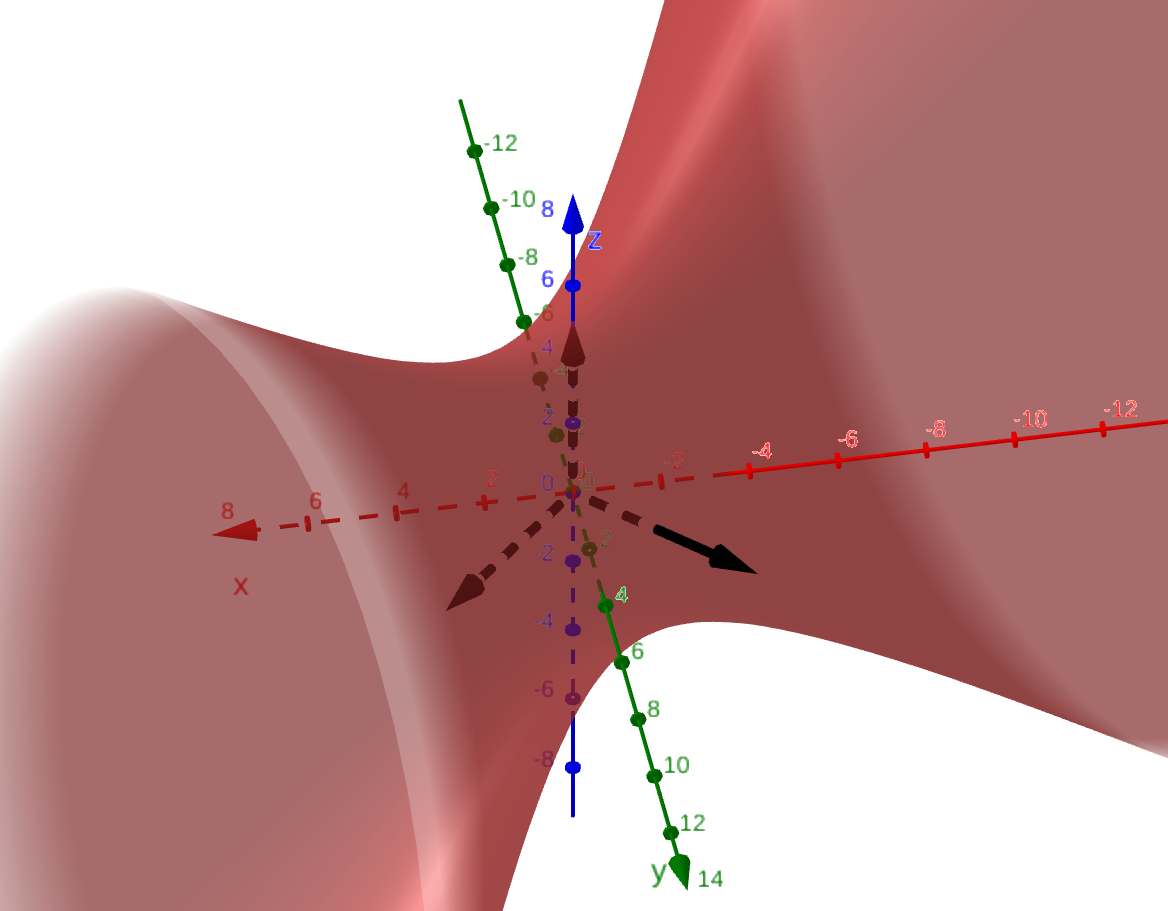
\includegraphics[height=200px]{rgr2.1.png}
    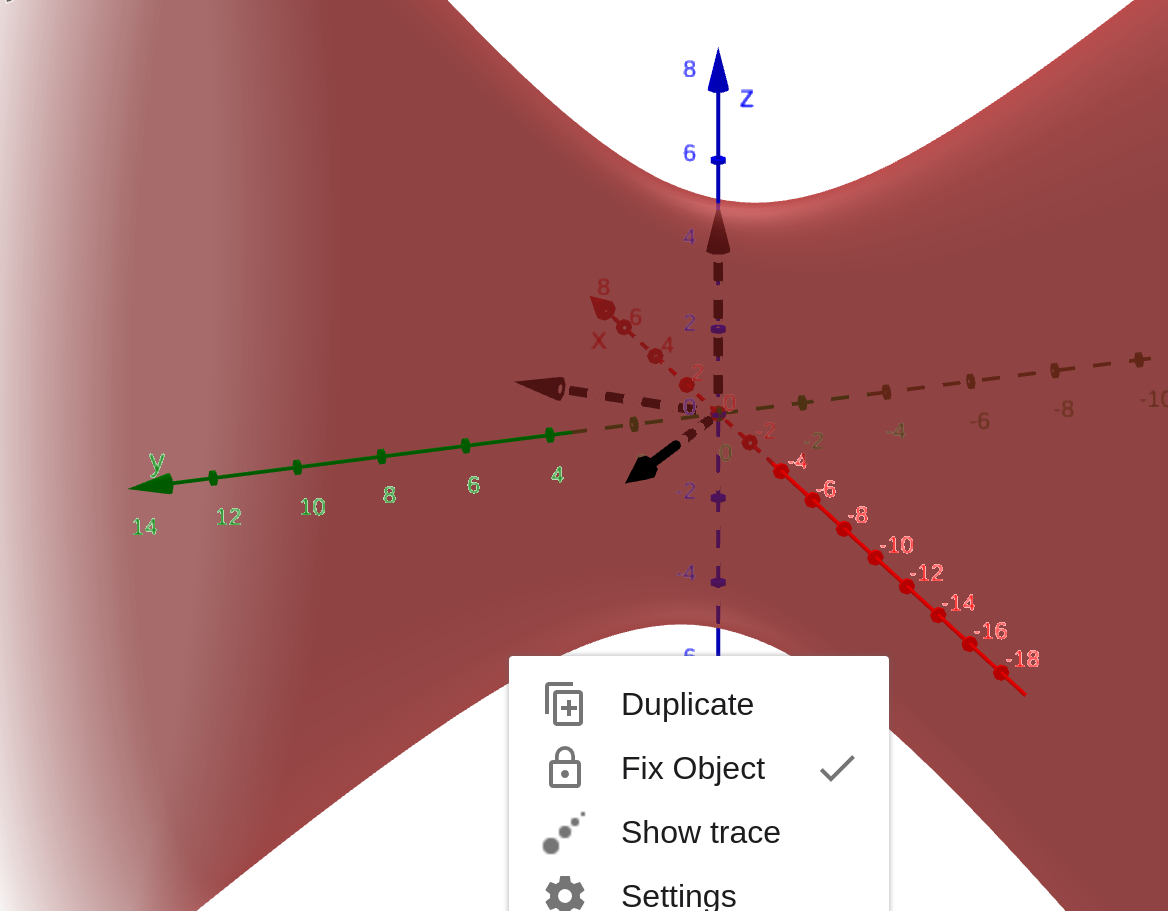
\includegraphics[height=200px]{rgr2.2.png}
    

% task 3
\newpage
    \section{Линейный оператор и спектральный анализ}
    \subsection{А}
    Изобразим подпространства $L_1$ и $L_2$ на графике. Подпространства представляют собой плоскости в трехмерном пространстве $R_3$  $L_1$ определяется системой уравнений: $x-y+z=0$ и $2x - 3y+4z=0$ и представляет собой пересечение 2 пересекающихся плоскостей в трехмерном пространстве $R_3$, то есть прямую. Найдем ее уравнение:\\
    $x-y+z=0$ \\
    $2x-3y+4z=0$\\
    $y = x+z$\\
    $2x-3x-3z+4z=0$\\
    $y=x+z$\\
    $x=z$\\
    $y=2z$\\
    $x=z$\\
    пусть $z=t$, тогда $x = t$, $y = 2t$; \\
    Получили направляющий вектор прямой $L_1$ $(1, 2, 1)$, также прямая проходит через точку $(0, 0, 0)$\\
    Тогда уравнение прямой имеет вид:\\
    $\frac{x}{1}=\frac{y}{2}=\frac{z}{1}$\\
    $L_2$ задано уравнением $2x+3y-4z=0$. Оно представляет собой плоскость в трехмерном пространстве. \\
    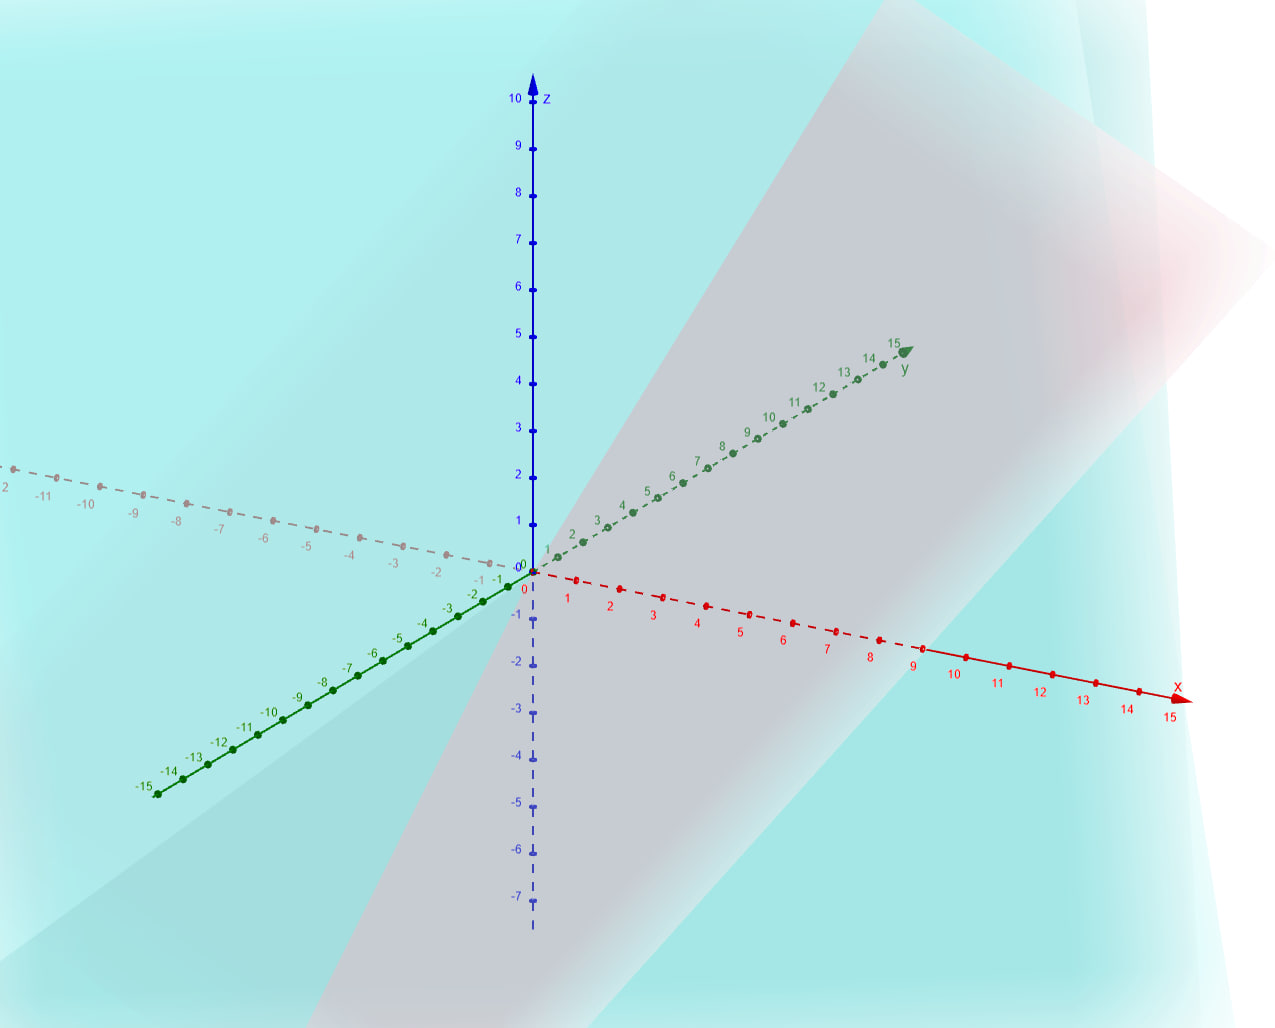
\includegraphics[height=200px]{rgr3.1.jpg}
    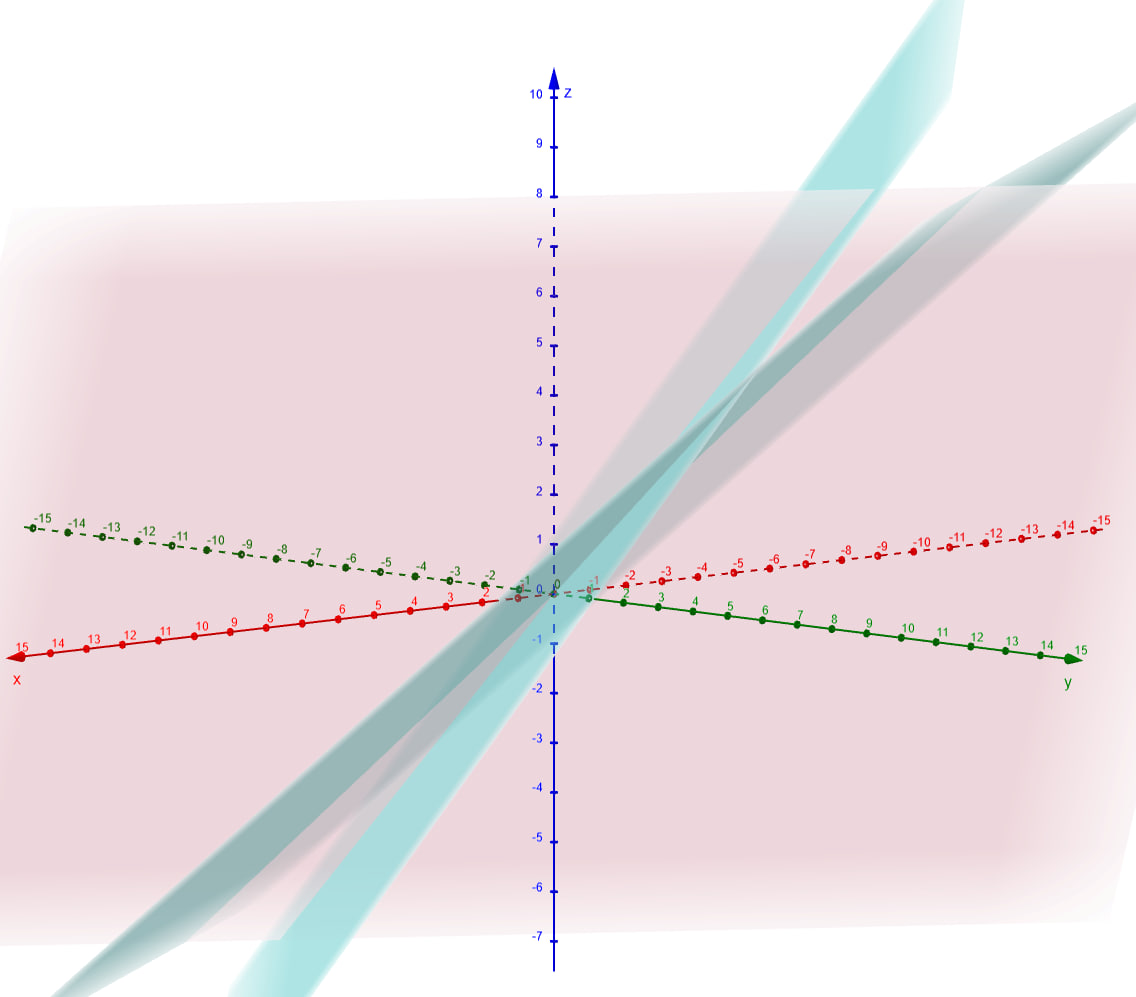
\includegraphics[height=200px]{rgr3.2.jpg}\\
    2) составим формулу для линейного оператора A - оператора проектирования пространства $R_3$ на подпространство $L_1$ параллельно $L_2$. \\
    Подпространство $L_1$ представляет собой прямую, а $L_2$ - плоскость. \\
    Поскольку оператор $A$ проецирует на $L_1$ параллельно $L_2$, проекция любого вектора на $L_1$ должна быть параллельна $L_2$. \\
    Пусть $v=(x, y, z)$ - произвольный вектор в пространстве $R_3$ . Тогда чтобы найти проекцию $M$ на $L_1$ параллельно $L_2$, нужно провести плоскость, параллельную $L_2$. Для этого в общее уравнение плоскости параллельной $L2$. \\
    $2x + 3y - 4z + d = 0$ подставим $x$, $y$, $z$, после чего найдем $d$. После этого остается найти точку пересечения этой плоскости с прямой $L_1$. \\
    Найденная точка $(x', y', z')$ и будет проекцией. \\
    Формула оператора $А: A(x, y, z)=(x', y', z')$\\
    3)Рассмотрим вектор $i =(1, 0, 0)$ \\
    Для начала найдем уравнение плоскости параллельной $L_2$: \\
    $2 \cdot 1 + 3 \cdot 0 - 4 \cdot 0 + d = 0$\\
    $d = -2$\\
    Найдем точку пересечения полученной плоскости и прямой $L_1$:\\
    $2x + 3y - 4z - 2 = 0$\\
    $\frac{x}{1}=\frac{y}{2}=\frac{z}{1}$\\
    Параметрическую форму $x=t$, $y=2t$, $z=t$ подставим в $2x + 3y - 4z - 2 = 0$:\\
    $2t + 6t - 4t - 2 = 0$\\
    $t = \frac{1}{2}$\\
    Искомая точка (проекция на $L_1$): $A(\frac{1}{2}, 1, \frac{1}{2})$\\
    \\
    Аналогично для вектора $j =(0, 1, 0)$:\\
    уравнение плоскости параллельной $L_2$:\\
    $2 \cdot 0 + 3 \cdot 1 - 4 \cdot 0 + d = 0$\\
    $d = -3$\\
    Найдем точку пересечения полученной плоскости и прямой $L_1$:\\
    $2x + 3y - 4z - 3 = 0$\\
    $\frac{x}{1}=\frac{y}{2}=\frac{z}{1}$\\
    Параметрическую форму $x=t$, $y=2t$, $z=t$ подставим в $2x + 3y - 4z - 3 = 0$:\\
    $2t + 6t - 4t - 3 = 0$\\
    $t = \frac{3}{4}$\\
    Искомая точка (проекция на $L_1$): $B(\frac{3}{4}, \frac{3}{2}, \frac{3}{4})$\\
    \\
    А также для вектора $k =(0,0,1)$:\\
    Для начала найдем уравнение плоскости параллельной $L_2$:\\
    $2 \cdot 0 + 3 \cdot 0 - 4 \cdot 1 + d = 0$\\
    $d = 4$\\
    Найдем точку пересечения полученной плоскости и прямой $L_1$:\\
    $2x + 3y - 4z + 4 = 0$\\
    $\frac{x}{1}=\frac{y}{2}=\frac{z}{1}$\\
    Параметрическую форму $x = t$, $y = 2t$, $z = t$ подставим в $2x + 3y - 4z + 4 = 0$:\\
    $2t + 6t - 4t + 4 = 0$\\
    $t = -1$\\
    Искомая точка (проекция на $L_1$): $C(-1, -2, -1)$\\
    Теперь чтобы найти матрицу оператора, решим уравнение $Av = v’$ для каждого из базисных векторов:\\
    \begin{equation*}
        \begin{pmatrix}
            a_1_1& a_1_2& a_1_3\\
            a_2_1& a_2_2& a_2_3\\
            a_3_1& a_3_2& a_3_3\\
            
        \end{pmatrix}
        \begin{pmatrix}
            1\\
            0\\
            0\\
        \end{pmatrix}
        =
        \begin{pmatrix}
            \frac{1}{2}\\
            1\\
            \frac{1}{2}\\
        \end{pmatrix}
    \end{equation*}
    \\
    \begin{equation*}
        \begin{pmatrix}
            a_1_1\\
            a_2_1\\
            a_3_1\\
        \end{pmatrix}
        =
        \begin{pmatrix}
            \frac{1}{2}\\
            1\\
            \frac{1}{2}\\
        \end{pmatrix}
    \end{equation*}
    \\
    \begin{equation*}
        \begin{pmatrix}
            a_1_1& a_1_2& a_1_3\\
            a_2_1& a_2_2& a_2_3\\
            a_3_1& a_3_2& a_3_3\\
            
        \end{pmatrix}
        \begin{pmatrix}
            0\\
            1\\
            0\\
        \end{pmatrix}
        =
        \begin{pmatrix}
            \frac{3}{4}\\
            \frac{3}{2}\\
            \frac{3}{4}\\
        \end{pmatrix}
    \end{equation*}
    \\
    \begin{equation*}
        \begin{pmatrix}
            a_1_1\\
            a_2_1\\
            a_3_1\\
        \end{pmatrix}
        =
        \begin{pmatrix}
            \frac{3}{4}\\
            \frac{3}{2}\\
            \frac{3}{4}\\
        \end{pmatrix}
    \end{equation*}
    \\
    \begin{equation*}
        \begin{pmatrix}
            a_1_1& a_1_2& a_1_3\\
            a_2_1& a_2_2& a_2_3\\
            a_3_1& a_3_2& a_3_3\\
            
        \end{pmatrix}
        \begin{pmatrix}
            0\\
            0\\
            1\\
        \end{pmatrix}
        =
        \begin{pmatrix}
            -1\\
            -2\\
            -1\\
        \end{pmatrix}
    \end{equation*}
    \\
    \begin{equation*}
        \begin{pmatrix}
            a_1_1\\
            a_2_1\\
            a_3_1\\
        \end{pmatrix}
        =
        \begin{pmatrix}
            -1\\
            2\\
            -1\\
        \end{pmatrix}
    \end{equation*}
    Матрица оператора имеет вид:
    \\
    \begin{equation*}
        A =
        \begin{pmatrix}
            \frac{1}{2}& \frac{3}{4}& -1\\
            1& \frac{3}{2}& -2\\
            \frac{1}{2}& \frac{3}{4}& -1\\    
        \end{pmatrix}
        \sim{~}
        \begin{pmatrix}
            1& \frac{3}{2}& -2\\
            0& 0& 0\\
            0& 0& 0\\
        \end{pmatrix}
    \end{equation*}
    \\
    4) Для начала найдем собственные числа оператора. Для этого решим
    уравнение $det(A - \lambda  \cdot  E)=0$
    \\
    \begin{equation*}
        A =
        \begin{vmatrix}
            1 - \lambda & \frac{3}{2}& -2\\
            0& 0-\lambda& 0\\
            0& 0& 0-\lambda\\    
        \end{vmatrix}
        = 0
    \end{equation*}
    \\
    $ 0 - \lambda(- \lambda + \lambda^2) + 0 = 0$\\
    $\lambda ^ 2 - \lambda ^ 3 = 0$\\
    $\lambda = 0; \lambda = 1 $ \\
    теперь найдем соответствующие им собственные векторы: \\
    1) $\lambda = 0$ \\
    \\
    \begin{equation*}
        \begin{pmatrix}
            1& \frac{3}{2}& -2\\
            0& 0& 0\\
            0& 0& 0\\    
        \end{pmatrix}
        \begin{pmatrix}
            $x_1$\\
            $x_2$\\
            $x_3$\\
        \end{pmatrix}
        =
        \begin{pmatrix}
            0\\
            0\\
            0\\
        \end{pmatrix}
    \end{equation*}
    $x_1 + \frac{3}{2}x_2 - 2x_3 = 0$ \\
    Общее решение: $x_1 = -\frac{3}{2}x_2 + 2x_3$,  $x_2 = a$,  $x_3 = b$ \\
    пусть $x_2 = 0$, $x_3 = 1$, тогда $x_1 = 2$ \\
    $v = (2, 0, 1)$ - собственный вектор \\
    2) $\lambda = 1$
    \\
    \begin{equation*}
        \begin{pmatrix}
            1-1& \frac{3}{2}& -2\\
            0& 0-1& 0\\
            0& 0& 0-1\\    
        \end{pmatrix}
        \begin{pmatrix}
            $x_1$\\
            $x_2$\\
            $x_3$\\
        \end{pmatrix}
        =
        \begin{pmatrix}
            0\\
            0\\
            0\\
        \end{pmatrix}
    \end{equation*}
    
    \\
    \begin{equation*}
        \begin{pmatrix}
            0& \frac{3}{2}& -2\\
            0& -1& 0\\
            0& 0& -1\\    
        \end{pmatrix}
        \begin{pmatrix}
            $x_1$\\
            $x_2$\\
            $x_3$\\
        \end{pmatrix}
        =
        \begin{pmatrix}
            0\\
            0\\
            0\\
        \end{pmatrix}
    \end{equation*}
    \\
    \begin{equation*}
        \begin{vmatrix}
            0& \frac{3}{2}& -2\\
            0& -1& 0\\
            0& 0& -1\\    
        \end{vmatrix}
        = 0 + (-1) \cdot (0 \cdot (-1) - 0 \cdot (-2)) + 0 = 0
    \end{equation*}
    Определитель равен 0, значит существует только тривиальное решение
    соответствующей системы, которое нас не устраивает.
    Чтобы решить задачу диагонализации матрицы, воспользуемся тем
    фактом, что матрица данного оператора в базисе из его собственных
    векторов является диагональной и содержит на главной диагонали
    собственные числа
    \\
    \begin{equation*}
        \begin{pmatrix}
            0& 0\\
            1& 0\\
        \end{pmatrix}
        \sim{~} 
        \begin{pmatrix}
            1 \\
            0 \\   
        \end{pmatrix}
    \end{equation*}
    \newpage
    5) \\
    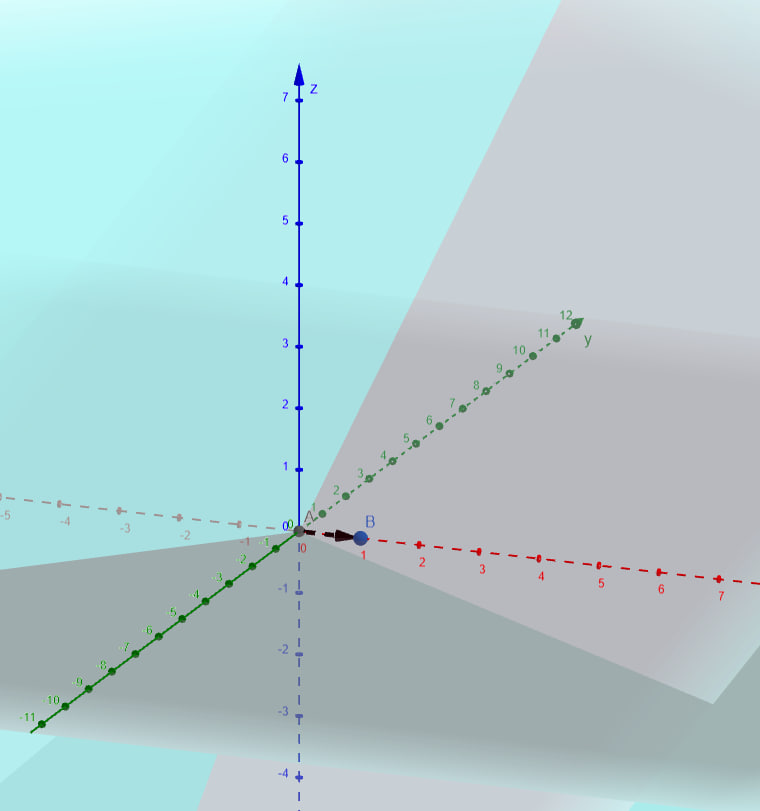
\includegraphics[height=200px]{rgr3.3.jpg}
    \\
    В данном случае базисом будет являться единичный вектор $(1, 0)^T$
    параллельный оси Ох. Через этот базис мы действительно сможем выразить координаты любого элемента подпространства $L_1$. \\ $L_1$ представляет из себя прямую, на которую под действием оператора $А$ проектируются элементы $R_3$, причем сама проекция является некоторой
    точкой на прямой, поэтому вектора $(1, 0)^T$ достаточно чтобы задать
    положение любой точки на данной прямой. Вектор соответствующий
    некоторой точке будет показывать ее смещение по оси Ox относительно
    начала координат. \\
    Б\\
    1) Для того чтобы выбрать базис в пространстве многочленов степени не
    выше второй с вещественными коэффициентами, нужно найти три
    линейно независимых многочлена, которые образуют базис этого
    пространства.\\
    Давайте рассмотрим многочлены, которые представлены в данной
    задаче:\\
    $f1(t) = 1$\\
    $f2(t) = t$\\
    $f3(t) = t^2$\\
    Проверим, являются ли такая система линейно независимой:\\
    Предположим, что существуют такие константы $c_1$, $c_2$, и $c_3$, хотя бы одна
    из которых не равна нулю, такие что:\\
    $c_1  \cdot  f1(t) + c_2  \cdot  f2(t) + c_3  \cdot  f3(t)=0$\\
    тогда $c_1 + c_2  \cdot  t+c_3  \cdot  t^2 = 0$\\
    Это равенство должно выполняться для всех значений $t$. Рассмотрим
    несколько значений $t$:\\
    При $t = 0$: $c_1 = 0$\\
    При $t = 1$: $c_1 + c_2 + c_3 = 0$\\
    При $t =-1$: $c_1 - c_2 + c_3 = 0$\\
    Теперь решим эту систему уравнений:\\
    Из первого уравнения $c_1 = 0$, а затем, подставив $c_1 = 0$ во второе и третье
    уравнения, получаем $c_2 = c_3 = 0$.\\
    Таким образом, многочлены $f1(t)=1$, $f2(t)=t$ и $f3(t)=t^2$ являются линейно
    независимыми.\\
    Таким образом, они образуют базис пространства многочленов степени
    не выше второй с вещественными коэффициентами.\\
    2) Чтобы убедиться, что отображение A является линейным оператором,
    нужно проверить два условия: \\
    1. Аддитивность:\\
    Пусть f(t) и g(t) - произвольные многочлены степени не выше второй.\\
    Тогда:\\
    $A(f + g) = (f + g)'' - 3(f + g)' + (f + g) = f '' + g'' - 3f ' - 3g' + f + g = (f '' - 3f ' + f) + (g'' -
    3g' + g) = A(f) + A(g)$ - выполняется\\
    2. Гомогенность:\\
    Пусть f(t) - произвольный многочлен степени не выше второй, $a \in R$ -
    произвольное число. Тогда:\\
    $A(af) = (af)'' - 3(af)' + af = a \cdot  f '' - 3 \cdot  a  \cdot  f ' + a \cdot  f = a(f '' - 3f ' + f) = a \cdot  A(f)$ -
    выполняется\\
    Таким образом, отображение А является линейным оператором.\\
    3) Чтобы найти матрицу оператора $A$ в выбранном базисе, мы должны
    вычислить образы базисных векторов под действием оператора $A$ и
    представить эти образы в координатном виде относительно выбранного
    базиса. \\
    1. Образ многочлена 1 под действием $A$:\\
    $A(1) = 1'' - 3  \cdot  1' + 1 = 1$\\
    2. Образ многочлена t под действием $A$:\\
    $A(t) = t'' - 3  \cdot  t' + t = -3 + t$\\
    3. Образ многочлена $t^2$ под действием $A$:\\
    $A(t^2) = (t^2)'' - 3  \cdot  (t^2)' + t^2 = 2t‘ - 6t + t^2 = 2 - 6t + t^2$\\
    Теперь представим каждый из этих образов в виде линейной
    комбинации базисных элементов $1$, $t$ и $t^2$:\\
    1. Образ многочлена $1$:\\
    $0 = 1  \cdot  1 + 0  \cdot  t + 0  \cdot  t^2 \Rightarrow (1, 0, 0)$\\
    2. Образ многочлена $t$:\\
    $-3 + t = -3  \cdot  1 + 1  \cdot  t + 0  \cdot  t^2 \Rightarrow (-3, 1, 0)$\\
    3. Образ многочлена $t^2$:\\
    $2 - 6t + t^2 = 2  \cdot  1 - 6  \cdot  t + 1  \cdot  t^2 \Rightarrow (2, -6, 1)$\\
    Теперь мы можем записать эти коэффициенты в матрицу, где каждый
    столбец представляет координаты образа соответствующего базисного
    вектора в выбранном базисе:
    \\
    \begin{equation*}
        A =
        \begin{pmatrix}
            1& -3& 2\\
            0& 1& -6\\
            0& 0& 1\\
        \end{pmatrix}
    \end{equation*}
    \\
    Это и есть матрица оператора $A$ в выбранном базисе. \\
    Чтобы найти ранг матрицы, заметим что она уже имеет ступенчатый вид,
    посчитаем количество ненулевых строк. Их две, поэтому ранг матрицы
    оператора $A$ равен $2$. \\
    4) Чтобы найти размерность ядра, мы должны решить уравнение $Af=0$,
    то есть найти все многочлены $f(t)$, для которых $Af=0$.\\
    $f'' - 3f' + f = 0 \\
    f(t) = a  \cdot  t^2 + b \cdot  t + c$\\
    $(a  \cdot  t^2 + b \cdot  t + c)'' + (a  \cdot  t^2 + b \cdot  t + c)’ + a  \cdot  t^2 + b \cdot  t + c = 0$\\
    $(2a  \cdot  t + b)’ + 2a  \cdot  t + b + a  \cdot  t^2 + b \cdot  t + c = 0$\\
    $2a + 2a  \cdot  t + b + a  \cdot  t^2 + b \cdot  t + c = 0$\\
    $a  \cdot  t^2 + (2a + b) t + (2a + b + c) = 0$\\
    Получили систему:\\
    \begin{equation*}
            \begin{cases}
                a = 0 \\
                2a + b = 0 \\
                2a + b + c = 0 \\
            \end{cases}
            \Rightarrow
            \begin{cases}
                a = 0 \\
                b = 0 \\
                c = 0 \\
            \end{cases}
        \end{equation*}
    $Ker A = {0 \cdot  t^2 + 0 \cdot  t + 0} = {(0, 0, 0)}$\\
    Размерность $Ker \; A$ равна $1$.\\
    Теперь чтобы найти размерность образа $Im \; A$ воспользуемся теоремой
    о размерностях ядра и образа: \\
    Сумма размерностей ядра и образа любого линейного отображения\\
    $A: V \to W$ равна размерности пространства прообразов: \\
    $dim \; ker \; A + dim \; im \; A = dim \; V$ \\
    в нашем случае $dim \; Ker \; A = 1$, $dim \; L = 3$ (так как $L$ пространство
    многочленов не выше $2$ степени)\\
    Тогда $dim \; Im \; A = dim \; L - dim \; Ker \; A = 3 - 1 = 2$\\
    5) Прежде всего найдем собственные числа оператора. Для этого решим
    уравнение $det(A - \lambda E)=0$ \\
    \begin{equation*}
        \begin{vmatrix}
            1 - \lambda& -3& 2\\
            0& 1 - \lambda& -6\\
            0& 0& 1 - \lambda \\
        \end{vmatrix}
        = 0
    \end{equation*}
    \\
    $-\lambda^3 + 3  \cdot  \lambda^2 - 3\lambda+1 = 0$ \\
    $-(\lambda - 1)^3 = 0$\\
    $\lambda = 1$ - собственное число
    Найдем собственный вектор соответствующий $\lambda = 1$
    \\
    \begin{equation*}
        \begin{pmatrix}
            1-1& -3& 2\\
            0& 1-1& -6\\
            0& 0& 1-1\\    
        \end{pmatrix}
        \begin{pmatrix}
            $x_1$\\
            $x_2$\\
            $x_3$\\
        \end{pmatrix}
        =
        \begin{pmatrix}
            0\\
            0\\
            0\\
        \end{pmatrix}
    \end{equation*}
    \\
    \begin{equation*}
        \begin{pmatrix}
            0& -3& 2\\
            0& 0& -6\\
            0& 0& 0\\    
        \end{pmatrix}
        \begin{pmatrix}
            $x_1$\\
            $x_2$\\
            $x_3$\\
        \end{pmatrix}
        =
        \begin{pmatrix}
            0\\
            0\\
            0\\
        \end{pmatrix}
    \end{equation*}
    получили систему уравнений: \\
    \begin{equation*}
            \begin{cases}
                -3  \cdot  x_2 + 2  \cdot  x_3 = 0 \\
                -6  \cdot  x_3 = 0 \\
            \end{cases}
        \end{equation*}
    Откуда общее решение: $x_1 = a$, $x_2 = 0$, $x_3 = 0$ \\
    пусть $x_1 = 1$, тогда $v = (1, 0, 0)^T$ - собственный вектор \\
    Размерность пространства собственных векторов равна количеству
    линейно независимых собственных векторов. В данном случае, у нас
    есть только один собственный вектор, так как кратность собственного
    значения $\lambda = 1$ равна 3, но для этого собственного значения существует
    только один линейно независимый собственный вектор. Следовательно,
    размерность пространства собственных векторов равна 1. \\
    Матрицу оператора нельзя диагонализировать, поскольку у нас есть
    только один линейно независимый собственный вектор для данной
    матрицы, в то время как для диагонализации нужно три линейно
    независимых собственных вектора (так как $dim \; L = 3$). Поэтому данную
    матрицу нельзя диагонализовать. \\
    6) Найдем образ вектора, соответствующего $p(t)$, с помощью умножения
    на матрицу оператора $A$: \\
    $p(t) = 3t^2 + t + 2 соответствует вектор (2, 1, 3)^T$ \\
    \begin{equation*}
        A * p(t) = 
        \begin{pmatrix}
            1& -3& 2\\
            0& 1& -6\\
            0& 0& 1\\
        \end{pmatrix}
        \begin{pmatrix}
            2\\
            1\\
            3\\
        \end{pmatrix}
        =
        \begin{pmatrix}
            5\\
            -17\\
            3\\
        \end{pmatrix}
    \end{equation*}
    $Ap(t) = (5, -17, 3) = 3* t^2 - 17 * t + 5$\\
    Проверим результат через дифференцирование: \\
$p(t) = 3t^2 + t + 2$ \\
$p’(t) = 6t + 1$ \\
$p(t)'' = 6$ \\
$Af = f'' - 3f′ + f = 6 - 3(6t + 1) + 3t^2 + t + 2 = 3t^2 -17t + 5 \Rightarrow (5, -17, 3)$\\
Таким образом матрица оператора была найдена верно.

    
% evaluation paper
\newpage
\[
\renewcommand{\arraystretch}{2}
\begin{tabular}{| c | c |}
 \hline
    \hugeУчастник & \hugeВклад в \% \\
 \hline
    \hugeКаренин Константин & \huge25 \\
 \hline
    \hugeГонин Сергей & \huge25 \\
 \hline
    \hugeТемиров Тимур & \huge25 \\
 \hline
    \hugeМалышева Алиса & \huge25 \\
 \hline
\end{tabular}
\]
\end{document}